\begin{tabularx}{\textwidth}{c c c c}

\textbf{Chess}
& \textbf{Shogi}
& \textbf{Go}
& \textbf{Atari} \\

\newgame
% Chess board
\scalebox{0.62}{\newgame \notationoff \showboard} &
% Shogi board
\scalebox{0.745}{
\begin{CJK}{UTF8}{min}
\begin{TAB}(e,0.5cm,0.5cm){|c|c|c|c|c|c|c|c|c|}{|c|c|c|c|c|c|c|c|c|}
\rotatebox[origin=c]{180}{香} & \rotatebox[origin=c]{180}{桂} & \rotatebox[origin=c]{180}{銀} & \rotatebox[origin=c]{180}{金} & \rotatebox[origin=c]{180}{玉} & \rotatebox[origin=c]{180}{金} & \rotatebox[origin=c]{180}{銀} & \rotatebox[origin=c]{180}{桂} & \rotatebox[origin=c]{180}{香}\\
 & \rotatebox[origin=c]{180}{飛} &  &  &  &  &  & \rotatebox[origin=c]{180}{角} & \\
\rotatebox[origin=c]{180}{歩} & \rotatebox[origin=c]{180}{歩} & \rotatebox[origin=c]{180}{歩} & \rotatebox[origin=c]{180}{歩} & \rotatebox[origin=c]{180}{歩} & \rotatebox[origin=c]{180}{歩} & \rotatebox[origin=c]{180}{歩} & \rotatebox[origin=c]{180}{歩} & \rotatebox[origin=c]{180}{歩}\\
 &  &  &  &  &  &  &  & \\
 &  &  &  &  &  &  &  & \\
 &  &  &  &  &  &  &  & \\
歩 & 歩 & 歩 & 歩 & 歩 & 歩 & 歩 & 歩 & 歩\\
 & 角 &  &  &  &  &  & 飛 & \\
香 & 桂 & 銀 & 金 & 玉 & 金 & 銀 & 桂 & 香\\
\end{TAB}
\end{CJK}
}%scalebox
&
% Go board.
\scalebox{0.195}{
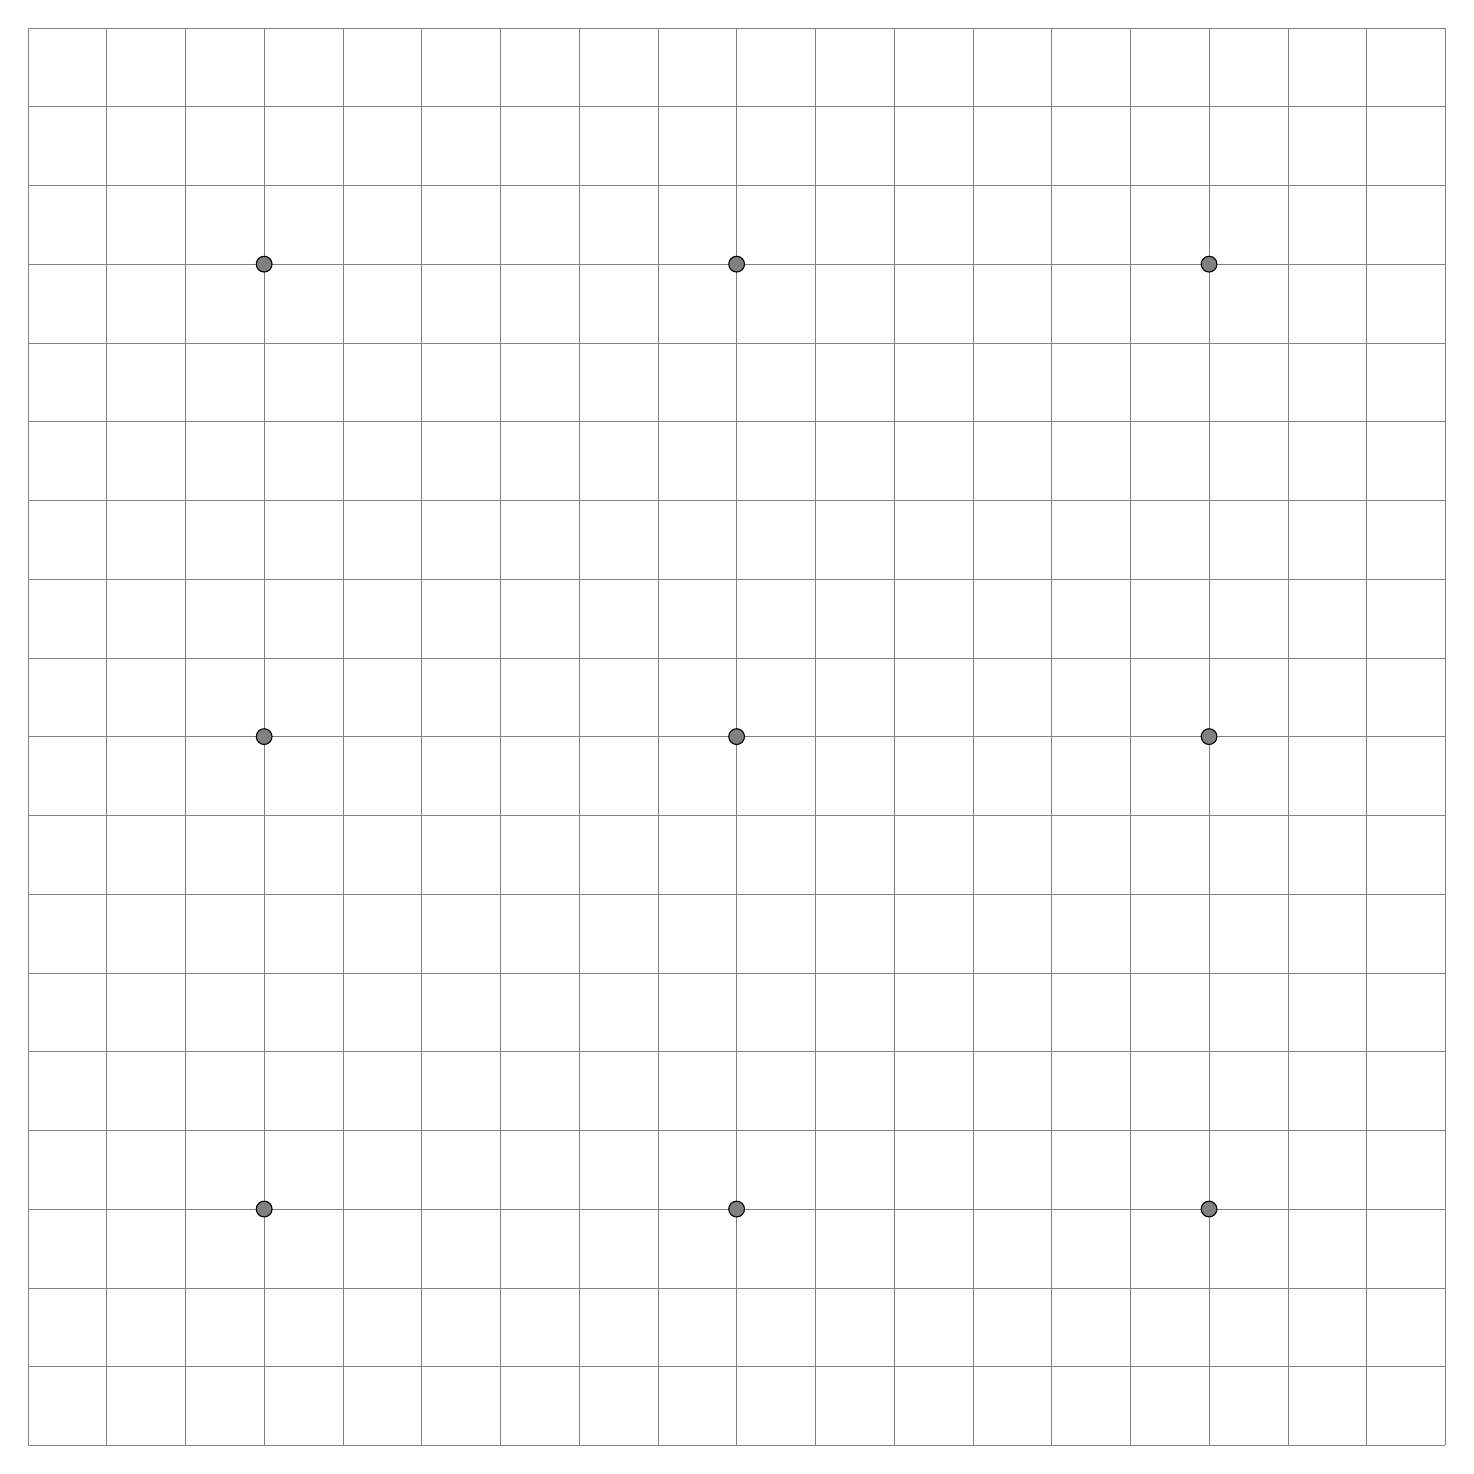
\begin{tikzpicture}
\draw[help lines] (0,0) grid (18,18);
\draw[fill=gray] (3,3) circle[radius=0.1];
\draw[fill=gray] (3,9) circle[radius=0.1];
\draw[fill=gray] (3,15) circle[radius=0.1];
\draw[fill=gray] (9,3) circle[radius=0.1];
\draw[fill=gray] (9,9) circle[radius=0.1];
\draw[fill=gray] (9,15) circle[radius=0.1];
\draw[fill=gray] (15,3) circle[radius=0.1];
\draw[fill=gray] (15,9) circle[radius=0.1];
\draw[fill=gray] (15,15) circle[radius=0.1];
\end{tikzpicture}
}
&
% Atari screenshot.
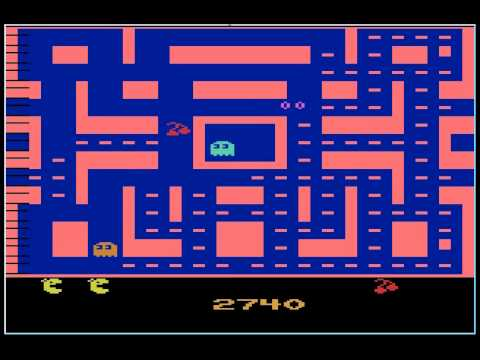
\includegraphics[width=0.219\textwidth,height=0.219\textwidth]{images/mspacman}
\\

\multicolumn{4}{c}{
  \hspace{-3.25em}
  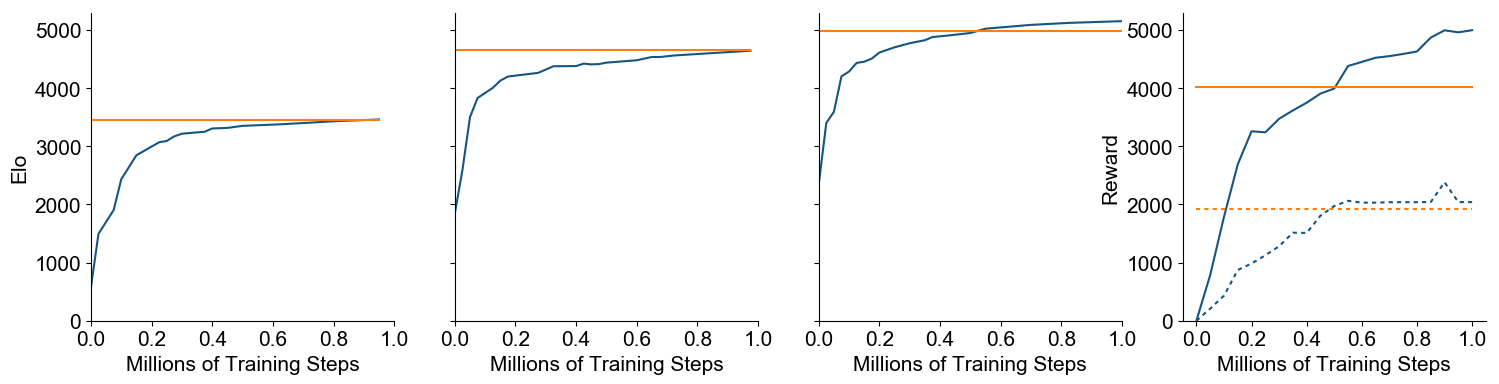
\includegraphics[width=\textwidth + 2.6em]{generated/training_plots}
}

\\

\end{tabularx}
